\documentclass{standalone}
\usepackage{tikz}
\usetikzlibrary{patterns, positioning}


\begin{document}
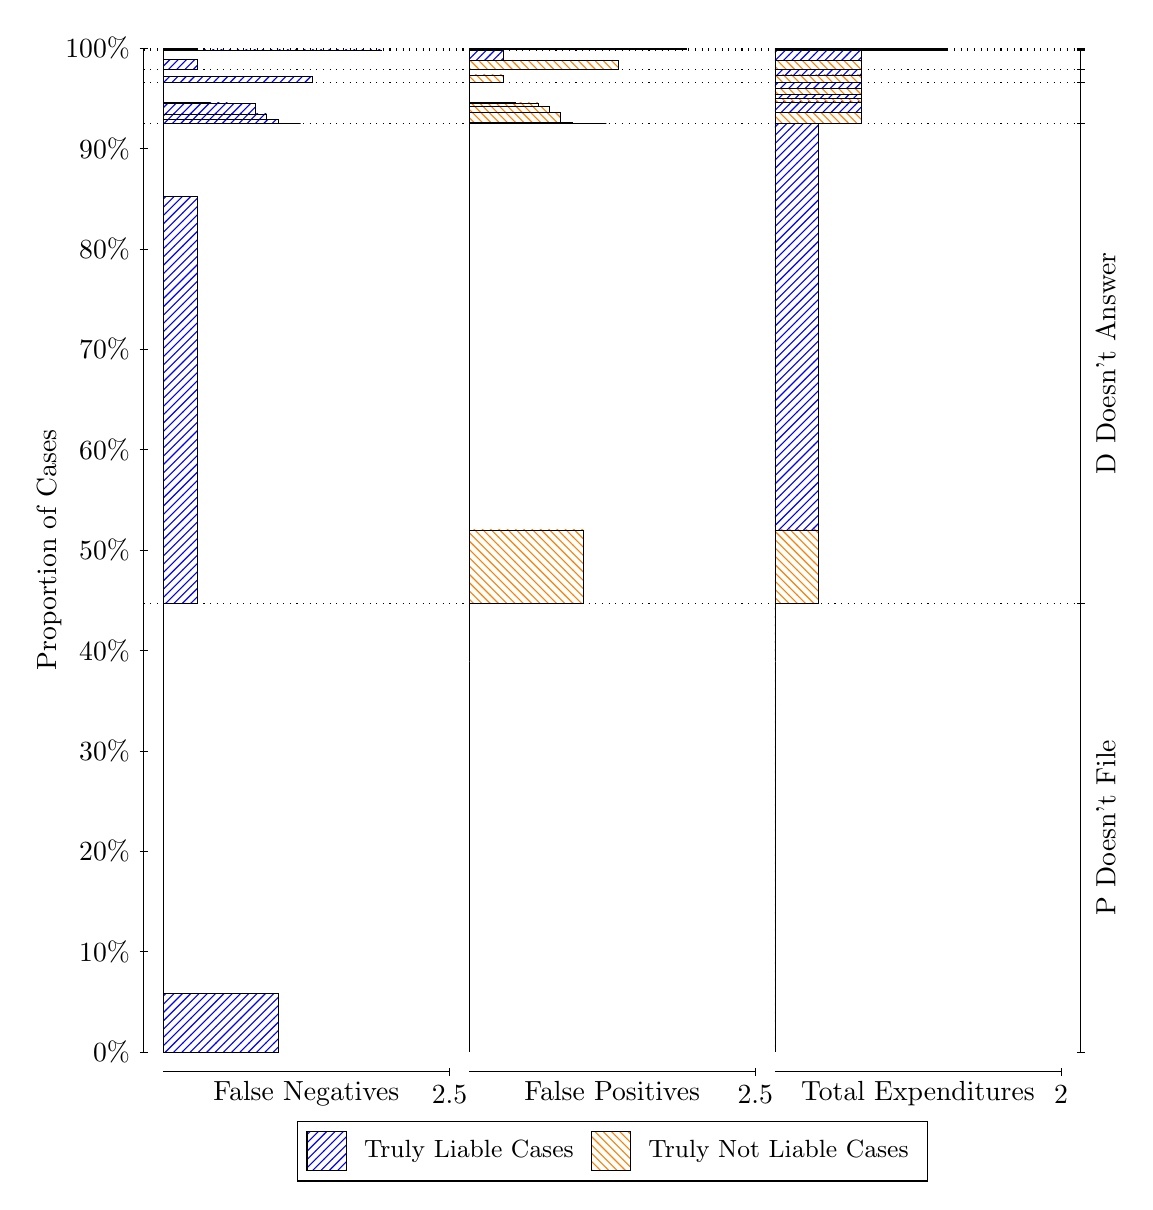
\begin{tikzpicture}
\draw[black, very thin] (1.5,1.75) -- (1.5,14.5);
\node[rotate=90, text=black, anchor=center] at (0.3, 8.125) {Proportion of Cases};
\draw[black, very thin] (1.45,1.75) -- (1.55,1.75);
\node[text=black, anchor=east] at (1.45, 1.75) {0\%};
\draw[black, very thin] (1.45,3.025) -- (1.55,3.025);
\node[text=black, anchor=east] at (1.45, 3.025) {10\%};
\draw[black, very thin] (1.45,4.3) -- (1.55,4.3);
\node[text=black, anchor=east] at (1.45, 4.3) {20\%};
\draw[black, very thin] (1.45,5.575) -- (1.55,5.575);
\node[text=black, anchor=east] at (1.45, 5.575) {30\%};
\draw[black, very thin] (1.45,6.85) -- (1.55,6.85);
\node[text=black, anchor=east] at (1.45, 6.85) {40\%};
\draw[black, very thin] (1.45,8.125) -- (1.55,8.125);
\node[text=black, anchor=east] at (1.45, 8.125) {50\%};
\draw[black, very thin] (1.45,9.4) -- (1.55,9.4);
\node[text=black, anchor=east] at (1.45, 9.4) {60\%};
\draw[black, very thin] (1.45,10.675) -- (1.55,10.675);
\node[text=black, anchor=east] at (1.45, 10.675) {70\%};
\draw[black, very thin] (1.45,11.95) -- (1.55,11.95);
\node[text=black, anchor=east] at (1.45, 11.95) {80\%};
\draw[black, very thin] (1.45,13.225) -- (1.55,13.225);
\node[text=black, anchor=east] at (1.45, 13.225) {90\%};
\draw[black, very thin] (1.45,14.5) -- (1.55,14.5);
\node[text=black, anchor=east] at (1.45, 14.5) {100\%};

\draw[black, very thin] (13.4,1.75) -- (13.4,14.5);
\draw[black, very thin] (13.35,1.75) -- (13.45,1.75);
\node[anchor=west] at (13.35, 1.75) {};
\draw[black, very thin] (13.35,7.4481) -- (13.45,7.4481);
\node[anchor=west] at (13.35, 7.4481) {};
\draw[black, very thin] (13.35,13.544) -- (13.45,13.544);
\node[anchor=west] at (13.35, 13.544) {};
\draw[black, very thin] (13.35,14.066) -- (13.45,14.066);
\node[anchor=west] at (13.35, 14.066) {};
\draw[black, very thin] (13.35,14.228) -- (13.45,14.228);
\node[anchor=west] at (13.35, 14.228) {};
\draw[black, very thin] (13.35,14.469) -- (13.45,14.469);
\node[anchor=west] at (13.35, 14.469) {};
\draw[black, very thin] (13.35,14.488) -- (13.45,14.488);
\node[anchor=west] at (13.35, 14.488) {};
\draw[black, very thin] (13.35,14.5) -- (13.45,14.5);
\node[anchor=west] at (13.35, 14.5) {};

\draw[black, very thin, pattern color=blue, pattern=north east lines] (1.75,1.75) rectangle (3.2033,2.4894);
\draw[black, very thin, pattern color=orange, pattern=north west lines] (1.75,2.4894) rectangle (1.75,7.4481);
\draw[black, very thin, pattern color=blue, pattern=north east lines] (1.75,7.4481) rectangle (2.186,12.611);
\draw[black, very thin, pattern color=orange, pattern=north west lines] (1.75,12.611) rectangle (1.75,13.544);
\draw[black, very thin, pattern color=blue, pattern=north east lines] (1.75,13.544) rectangle (3.494,13.544);
\draw[black, very thin, pattern color=blue, pattern=north east lines] (1.75,13.544) rectangle (3.3487,13.546);
\draw[black, very thin, pattern color=blue, pattern=north east lines] (1.75,13.546) rectangle (3.2033,13.59);
\draw[black, very thin, pattern color=blue, pattern=north east lines] (1.75,13.59) rectangle (3.058,13.59);
\draw[black, very thin, pattern color=blue, pattern=north east lines] (1.75,13.59) rectangle (3.058,13.663);
\draw[black, very thin, pattern color=blue, pattern=north east lines] (1.75,13.663) rectangle (2.9127,13.797);
\draw[black, very thin, pattern color=blue, pattern=north east lines] (1.75,13.797) rectangle (2.7673,13.801);
\draw[black, very thin, pattern color=blue, pattern=north east lines] (1.75,13.801) rectangle (2.622,13.803);
\draw[black, very thin, pattern color=blue, pattern=north east lines] (1.75,13.803) rectangle (2.4767,13.804);
\draw[black, very thin, pattern color=blue, pattern=north east lines] (1.75,13.804) rectangle (2.3313,13.805);
\draw[black, very thin, pattern color=orange, pattern=north west lines] (1.75,13.805) rectangle (1.75,14.066);
\draw[black, very thin, pattern color=blue, pattern=north east lines] (1.75,14.066) rectangle (3.6393,14.135);
\draw[black, very thin, pattern color=orange, pattern=north west lines] (1.75,14.135) rectangle (1.75,14.228);
\draw[black, very thin, pattern color=blue, pattern=north east lines] (1.75,14.228) rectangle (2.186,14.357);
\draw[black, very thin, pattern color=orange, pattern=north west lines] (1.75,14.357) rectangle (1.75,14.469);
\draw[black, very thin, pattern color=blue, pattern=north east lines] (1.75,14.469) rectangle (4.5113,14.475);
\draw[black, very thin, pattern color=orange, pattern=north west lines] (1.75,14.475) rectangle (1.75,14.488);
\draw[black, very thin, pattern color=blue, pattern=north east lines] (1.75,14.488) rectangle (2.186,14.494);
\draw[black, very thin, pattern color=orange, pattern=north west lines] (1.75,14.494) rectangle (1.75,14.5);
\draw[black, very thin, pattern color=orange, pattern=north west lines] (5.6333,1.75) rectangle (5.6333,6.7086);
\draw[black, very thin, pattern color=blue, pattern=north east lines] (5.6333,6.7086) rectangle (5.6333,7.4481);
\draw[black, very thin, pattern color=orange, pattern=north west lines] (5.6333,7.4481) rectangle (7.0867,8.381);
\draw[black, very thin, pattern color=blue, pattern=north east lines] (5.6333,8.381) rectangle (5.6333,13.544);
\draw[black, very thin, pattern color=orange, pattern=north west lines] (5.6333,13.544) rectangle (7.3773,13.544);
\draw[black, very thin, pattern color=orange, pattern=north west lines] (5.6333,13.544) rectangle (7.232,13.545);
\draw[black, very thin, pattern color=orange, pattern=north west lines] (5.6333,13.545) rectangle (7.0867,13.547);
\draw[black, very thin, pattern color=orange, pattern=north west lines] (5.6333,13.547) rectangle (6.9413,13.551);
\draw[black, very thin, pattern color=orange, pattern=north west lines] (5.6333,13.551) rectangle (6.796,13.685);
\draw[black, very thin, pattern color=orange, pattern=north west lines] (5.6333,13.685) rectangle (6.6507,13.758);
\draw[black, very thin, pattern color=orange, pattern=north west lines] (5.6333,13.758) rectangle (6.5053,13.802);
\draw[black, very thin, pattern color=orange, pattern=north west lines] (5.6333,13.802) rectangle (6.36,13.804);
\draw[black, very thin, pattern color=orange, pattern=north west lines] (5.6333,13.804) rectangle (6.2147,13.805);
\draw[black, very thin, pattern color=blue, pattern=north east lines] (5.6333,13.805) rectangle (5.924,13.806);
\draw[black, very thin, pattern color=blue, pattern=north east lines] (5.6333,13.806) rectangle (5.7787,13.806);
\draw[black, very thin, pattern color=blue, pattern=north east lines] (5.6333,13.806) rectangle (5.6333,14.066);
\draw[black, very thin, pattern color=orange, pattern=north west lines] (5.6333,14.066) rectangle (6.0693,14.158);
\draw[black, very thin, pattern color=blue, pattern=north east lines] (5.6333,14.158) rectangle (5.6333,14.228);
\draw[black, very thin, pattern color=orange, pattern=north west lines] (5.6333,14.228) rectangle (7.5227,14.34);
\draw[black, very thin, pattern color=blue, pattern=north east lines] (5.6333,14.34) rectangle (6.0693,14.469);
\draw[black, very thin, pattern color=orange, pattern=north west lines] (5.6333,14.469) rectangle (6.0693,14.481);
\draw[black, very thin, pattern color=blue, pattern=north east lines] (5.6333,14.481) rectangle (5.6333,14.488);
\draw[black, very thin, pattern color=orange, pattern=north west lines] (5.6333,14.488) rectangle (8.3947,14.493);
\draw[black, very thin, pattern color=blue, pattern=north east lines] (5.6333,14.493) rectangle (6.9413,14.5);
\draw[black, very thin, pattern color=orange, pattern=north west lines] (9.5167,1.75) rectangle (9.5167,6.7086);
\draw[black, very thin, pattern color=blue, pattern=north east lines] (9.5167,6.7086) rectangle (9.5167,7.4481);
\draw[black, very thin, pattern color=orange, pattern=north west lines] (9.5167,7.4481) rectangle (10.062,8.381);
\draw[black, very thin, pattern color=blue, pattern=north east lines] (9.5167,8.381) rectangle (10.062,13.544);
\draw[black, very thin, pattern color=orange, pattern=north west lines] (9.5167,13.544) rectangle (10.607,13.68);
\draw[black, very thin, pattern color=blue, pattern=north east lines] (9.5167,13.68) rectangle (10.607,13.817);
\draw[black, very thin, pattern color=orange, pattern=north west lines] (9.5167,13.817) rectangle (10.607,13.864);
\draw[black, very thin, pattern color=blue, pattern=north east lines] (9.5167,13.864) rectangle (10.607,13.91);
\draw[black, very thin, pattern color=orange, pattern=north west lines] (9.5167,13.91) rectangle (10.607,13.988);
\draw[black, very thin, pattern color=blue, pattern=north east lines] (9.5167,13.988) rectangle (10.607,14.066);
\draw[black, very thin, pattern color=orange, pattern=north west lines] (9.5167,14.066) rectangle (10.607,14.158);
\draw[black, very thin, pattern color=blue, pattern=north east lines] (9.5167,14.158) rectangle (10.607,14.228);
\draw[black, very thin, pattern color=orange, pattern=north west lines] (9.5167,14.228) rectangle (10.607,14.34);
\draw[black, very thin, pattern color=blue, pattern=north east lines] (9.5167,14.34) rectangle (10.607,14.469);
\draw[black, very thin, pattern color=orange, pattern=north west lines] (9.5167,14.469) rectangle (11.697,14.481);
\draw[black, very thin, pattern color=blue, pattern=north east lines] (9.5167,14.481) rectangle (11.697,14.488);
\draw[black, very thin, pattern color=orange, pattern=north west lines] (9.5167,14.488) rectangle (11.697,14.493);
\draw[black, very thin, pattern color=blue, pattern=north east lines] (9.5167,14.493) rectangle (11.697,14.5);
\draw[black, dotted] (1.5,7.4481) -- (13.4,7.4481);
\draw[black, dotted] (1.5,13.544) -- (13.4,13.544);
\draw[black, dotted] (1.5,14.066) -- (13.4,14.066);
\draw[black, dotted] (1.5,14.228) -- (13.4,14.228);
\draw[black, dotted] (1.5,14.469) -- (13.4,14.469);
\draw[black, dotted] (1.5,14.488) -- (13.4,14.488);
\draw[black, very thin] (1.75,1.5) -- (5.3833,1.5);
\node[text=black, anchor=north] at (3.5667, 1.5) {False Negatives};
\draw[black, very thin] (5.3833,1.45) -- (5.3833,1.55);
\node[text=black, anchor=north] at (5.3833, 1.45) {2.5};

\draw[black, very thin] (5.6333,1.5) -- (9.2667,1.5);
\node[text=black, anchor=north] at (7.45, 1.5) {False Positives};
\draw[black, very thin] (9.2667,1.45) -- (9.2667,1.55);
\node[text=black, anchor=north] at (9.2667, 1.45) {2.5};

\draw[black, very thin] (9.5167,1.5) -- (13.15,1.5);
\node[text=black, anchor=north] at (11.333, 1.5) {Total Expenditures};
\draw[black, very thin] (13.15,1.45) -- (13.15,1.55);
\node[text=black, anchor=north] at (13.15, 1.45) {2};

\node[text=black, centered, rotate=90] at (13.72, 4.599) {P Doesn't File};
\node[text=black, centered, rotate=90] at (13.72, 10.496) {D Doesn't Answer};






\draw (7.449999999999999,1.5) node[draw=none] (baseCoordinate) {};
\begin{scope}[align=center]
        \matrix[scale=0.5, draw=black, below=0.5cm of baseCoordinate, nodes={draw}, column sep=0.1cm]{
            \node[rectangle, draw, minimum width=0.5cm, minimum height=0.5cm, pattern color=blue, pattern=north east lines] {}; &
            \node[draw=none, font=\small, text=black] (B) {Truly Liable Cases}; &
            \node[rectangle, draw, minimum width=0.5cm, minimum height=0.5cm, pattern color=orange, pattern=north west lines] {}; &
            \node[draw=none, font=\small, text=black] (B) {Truly Not Liable Cases}; \\
            };
\end{scope}

\end{tikzpicture}
\end{document}